%!TEX root = ../dokumentation.tex

\chapter{Datengenerierung}

\section{Random Sampling}

Mit Random Sampling ist eine Zufallsstichprobe gemeint bei der eine Stichprobe aus einer Grundgesamtheit $X$ mit $n$ Elementen gezogen wird. Seien die Elemente der Grundgesamheit $x_1,x_2,\dots,x_n-1,x_n$, dann unterliegt die Auswahl eines Elements $x \in M$ einem Auswahlverfahren, das angibt mit welcher Auftrittswahrscheinlichkeit $P(x)$ ein Element in die Stichprobe $N$ gelangen kann \cite{RandomSampling}.
Es gelten die Bedingungen:
\begin{itemize}
    \item $P(x) > 0$ (Positivität)
    \item $\sum_{i=1}^{n}P(x_i)=1$ (Vollständigkeit)
\end{itemize}

Bei einer einfachen Zufallsstichprobe handelt es sich um die Auswahl einer Teilmenge einer statistischen Population, bei der jedes Element die gleiche Wahrscheinlichkeit $P(x)=\frac{1}{\lvert M \rvert}=\frac{1}{n}$ hat, ausgewählt zu werden. Zudem darf eine Ziehung aus einer Gesamtmenge nicht die nachfolgenden Ziehungen beeinflussen, weil sie unabhängig voneinander erfolgen müssen \cite{RandomSampling}. Übertragen auf das typische Urnenexperiment der Stochastik, kommt es bei einer einfachen Zufallsstichprobe zu einer Ziehung mit Zurücklegen.

Für die Generation von Trainingsdaten ist das Random Sampling von großer Bedeutung, weil nur durch Einbeziehung einer Zufallskomponente neue Datensätze generiert werden können. Genau genommen handelt es sich bei der gewählten Vorgehensweise des Graph-Editors nur um eine Ziehung von einem einzigen Element. Der Grund hierfür liegt darin, dass nicht pro Feature in der $n$-zeiligen Ergebnismenge auch gleich $n$ Elemente auf einmal aus der Grundgesamtheit gezogen werden, sondern in jedem Durchgang ein Element mit einer bestimmten Wahrscheinlichkeit gezogen wird, welches dann in weitere Berechnungen von anderen Features einfließen kann. Die Knoten können sich so auf eine einelementige Ziehung beschränken, welche dann beliebig oft ausgeführt weden kann, je nachdem wie viele Datensätze generiert werden sollen.

Sollen beispielsweise zufällig ortspezfische Personendaten generiert werden, könnte die Herausforderung bestehen Daten von hunderten Personen aus nur vier Wohnorten zu generieren. Jeder Person soll dabei ein Wohnort zugewiesen werden, der zufällig bestimmt wird. Ist die Wahrscheinlichkeit für die Auswahl eines Wohnorts gleich groß, so ergibt sich eine einfache Zufallsstichprobe. Oft genügt eine Gleichverteilung jedoch nicht, um eine Zufallsvariable zu modellieren, weil in der Realität andere Faktoren die Wahrscheinlichkeitsverteilung beeinflussen. Will man bezogen auf die Generation von Personendaten beispielsweise Größen generieren, wird eine Normal-, auch Gauß- oder Glockenverteilung benötigt. Es kann auch sein, dass die Wahrscheinlichkeitsverteilung so spezifisch definiert ist, dass sie nicht mit einer einzigen Funktion dargestellt werden kann.

In den folgenden Kapiteln soll auf die folgenden Fälle und deren Umsetzung eingegangen werden.
\begin{enumerate}
    \item Generation von gleichverteilten Zufallszahlen
    \item Generation von Zufallszahlen einer vorgegeben Wahrscheinlichkeitsverteilung
    \item Generation von Zufallszahlen einer benutzerdefinierten Wahrscheinlichkeitsverteilung
\end{enumerate}

\subsection{Generation von gleichverteilten Zufallszahlen}

Für die einfache Zufallsstichprobe kann das Problem auf die Frage reduziert werden, wie eine gleichverteilte Zufallszahl in dem Intervall $I=[0;1]$ generiert werden kann. Diese Zufallszahl kann dann auf ein beliebiges Intervall transformiert werden. Sei $x_1$ eine gleichverteilte Zufallszahl im Intervall $I_1=[0;1]$ und seien $a$, $b$ Grenzen des Intervalls $I_2=[a;b]$, so ist die Zufallszahl $x_2$ im intervall $I_2$ bestimmt durch $x_2=x_1 \cdot b+a$ \cite{prng}. Durch das Runden auf die Einerstelle, können so auch diskrete Werte resultieren.

Um gleichverteilte Zufallszahlen generieren zu können, wird ein \ac{PRNG} verwendet. Ein \ac{PRNG} oder auch Zufallszahlengenerator stellt einen Algorithmus dar, der eine Sequenz von Zufallszahlen generiert. Es handelt sich bei den generierten Zahlen um Pseudo-Zufallszahlen, weil das zugrundeliegende Verfahren deterministisch implementiert ist \cite{prng}. Bei gleichen Eingangsparametern ist auch immer das gleiche Ergebnis zu erwarten. 

Der entscheidende Parameter eines \ac{PRNG} ist der sogenannte Seed. Der Seed ist ein Startwert, der bei dem allerersten Aufruf des \ac{PRNG} initial gesetzt wird. Aufbauend auf diesem Seed können alle weiteren Zufallszahlen generiert werden. Jeder generierte Wert wird als neuer Startwert für das Verfahren verwendet. Da der mögliche Wertebereich durch eine festgelegte Speichergröße begrenzt ist, muss zwangsläufig irgendwann eine Zahl generiert werden, die bereits in der Sequenz aufgetaucht ist. Weil sich die generierte Sequenz wiederholt, ist der Zufallszahlengenerator periodisch. Simple lineare Kongruenzgeneratoren durchlaufen den Wertebereich im besten Fall einmal pro Periode, weil sie mit nur einem Seed als initialen Wert arbeiten \cite{prng}. Andere \ac{PRNG} wie z. B. der Mersenne-Twister arbeiten mit mehreren Seeds, wodurch eine erheblich größere Periodenlänge erreicht werden kann.

Ein Algorithmus kann Pseudo-Zufallszahlen generieren, welche sich nur in einer bestimmten Anwendung nicht von echten Zufallszahlen unterscheiden lassen. Manche Generatoren sind deshalb für bestimmte Anwendungen gut geeignet und andere wiederum nicht. Müssen beispielsweise lange Sequenzen von Zufallszahlen generiert werden, ist ein linearer Kongruenzgenerator nicht zu empfehlen. Hingegen wäre er bei einer performanten Generation von kurzen Sequenzen eher geeignet. Echte Zufallszahlen verhalten sich immer gleich und bieten hohe Güte. Zur Generation von echten Zufallszahlen kommen pyhsikalische Zufallszahlengeneratoren zum Einsatz, die die naturgemäße Zufälligkeit von physikalischen Prozessen zu Nütze machen. Beispiele für solche physikalischen Prozesse sind thermisches Rauschen eines Widerstands und radioaktive Zerfallsvorgänge \cite{prng}. Logischerweise ist dann die Benutzung eines Seeds und damit die Reproduzierbarkeit von physikalischen Zufallszahlengeneratoren nicht gegeben.

Die Möglichkeit einen Seed verwenden zu können, hat allerdings den großen Vorteil der Reproduzierbarkeit von Ergebnissen, weshalb die Verwendung von echten Zufallszahlen für den \ac{MLTDG} unpassend ist. Gerade bei der Erstellung von komplexen Zusammenhängen innerhalb der Applikation soll ein Neustart der Generation nach kleinen Veränderungen nicht komplett neue Daten generieren. Dem Benuter soll es möglich sein benutzerdefinierte Zufallsvariablen mit einem Seed zu versehen, um gleiche Ausgangswerte erhalten zu können.

Vorteile von Seeds:
\begin{itemize}
    \item Portabilität: Durch Speicherung der Seed-Werte bei einem Projektexport, werden bei unverändertem Projekt immer gleiche Trainingsdaten generiert, sodass das Projekt geteilt und wiederverwendet werden kann. 
    \item Debugging: Werden unerwartete Trainingsdaten generiert, können mithilfe von Seeds einzelne Änderungen vorgenommen werden, sodass die neuen Daten mit den letzten abgeglichen werden können. Aufgedeckte Singularitäten können so aufgedeckt und reproduziert werden. 
\end{itemize}

Es gibt einige JavaScript-Bibiliotheken, die \ac{PRNG}s bereits implementieren. Die Auswahl der Bibiliothek ist auf Chance.js aus den folgenden Gründen gefallen:
\begin{itemize}
    \item Einfache Nutzung durch die Verfügbarkeit als NPM-Package
    \item Ausführliche Dokumentation
    \item Verwendung eines Seeds
    \item Hohe Qualität durch integrierte Unit-Tests
\end{itemize}

\subsection{Generation von Zufallszahlen einer vorgegeben Wahrscheinlichkeitsverteilung}

Oft unterliegen Zufallsvariablen keiner gleichverteilten, sondern einer anderen Wahrscheinlichkeitsverteilung wie zum Beispiel die Normalverteilunge oder Exponentialverteilung. In diesem Fall wird ein Verfahren benötigt, um aus einer gleichverteilten Zufallszahl eine Zufallszahl einer anderen Wahrscheinlichkeitsverteilung zu generieren.

Die Inversionsmethode ist ein Algorithmus, der bei mehrfachem Aufruf eine Sequenz von Zufallszahlen $x_0, x_1, x2$ generiert, die einem vorgegeben stochastischem Modell entspringen. Der Algorithmus beschäftigt sich mit dem Problem, eine beliebige Verteilung auf $\mathbb{R}$ abzubilden. Neben der Verteilungsfunktion ist eine Voraussetzung für die Inversionsmethode ein vorhandener Zufallszahlengenerator, der gleichverteilte Zufallszahlen im Intervall $I=[0,1]$ generieren kann \cite{Inversionsmethode}. Hierfür kann der \ac{PRNG} der Bibliothek Chart.js aus dem letzten Kapitel herangezogen werden.

Das Inversionsprinzip ist wie folgt definiert:\\
Es sei $F$ eine Verteilungsfunktion und $U$ eine $U(0,1)$-verteilte Zufallsvariable.\\
Dann gilt \cite{Inversionsmethode}: $Y = F^{-1}(U)$ hat die Verteilungsfunktion $F$, d. h.
$$P(Y \le t)=F(t),t \in \mathbb{R}$$

Das Hauptproblem ist damit die Bestimmung der Inversen einer Verteilungsfunktion. Da nicht jede Funktion umkehrbar ist, kann dieses Verfahren nur für bestimmte Wahrscheinlichkeitsfunktionen verwendet werden. Im Folgenden wird die Berechnung der Inversen für die im \ac{MLTDG} relevanten Verteilungen erläutert.

Die Exponentialverteilung ist eine stetige Wahrscheinlichkeitsverteilung über der Menge der positiven reellen Zahlen. Sie wird häufig verwendet, um die Dauer von Zeitintervallen zu modellieren:
\begin{itemize}
    \item Dauer eines Telefongesprächs
    \item Alter von Lebewesen
    \item Zeitspanne zwischen zwei Anrufen
    \item Lebensdauer von Geräten
\end{itemize}
Die Verteilungsfunktion der Exponentialverteilung 
$$F(X)=1-e^-\lambda x$$
berechnet die Auftrittswahrscheinlichkeit des nächsten Ereignisses im Intervall $[0;x]$.\\
Die Inverse ist definiert durch
$$x=F^{-1}(y)=-\frac{1}{\lambda}ln(1-y)$$

Die Inversionsmethode gelingt nicht immer, weil nicht jede Funktion auch umkehrbar ist. Nur für Funktionen von denen die Inverse gebildet werden kann, kann die Inversionsmethode zur Erzeugung von Zufallszahlen für eine vorgegebene Verteilung eingesetzt werden. Eine weitere wichtige Verteilung ist die Normalverteilung für die unmittelbar keine Inverse ermittelt werden kann. 

Die Normalverteilung ist eine stetige Wahrscheinlichkeitsverteilung mit großer Bedeutung, weil sich viele Prozesse natur-, wirtschafts- und ingenieurswissenfschaftlicher Herkunft entweder exakt oder näherungsweise mit ihr darstellen lassen.\\ 
Die Normalverteilung $\mathcal{N}(\mu,\sigma ^2)$ ist definiert durch die zwei Parameter: 
\begin{itemize}
    \item $\mu$: Erwartungswert
    \item $\sigma^2$: Varianz mit der Standardabweichung $\sqrt{\sigma^2}=\sigma$
\end{itemize}
Die Kurve der Normalverteilung wird mit der Dichtefunktion
\medskip
$$f(x,\mu,\sigma^2)=\frac{1}{\sigma\sqrt{2\pi}}e^{-\frac{1}{2}(\frac{x-\mu}{\sigma})^2}$$
\medskip
dargestellt \cite{Inversionsmethode}.

Es wurden einige Algorithmen entwickelt, um näherungsweise normalverteilte Zufallszahlen zu generieren. Im Folgenden werden einige relevante Algorithmen zur Vollständigkeit aufgezählt aber auf sie nicht näher eingegangen:
\begin{itemize}
    \item Ziggurat-Algorithmus
    \item Box-Muller-Methode
    \item Polar-Methode
\end{itemize}

Die verwendete Bibliothek Chance.js implementiert die Polar-Methode von George Marsaglia und Thomas A. Die Polar-Methode basiert auf der Box-Muller-Methode und verbessert verbessert sie, indem die Berechnung von trigonometrischen Funktionen umgangen wird. Statt euklidischen Koordinaten werden Polar-Koordinaten verwendet \cite{polarmethode}.

\subsection{Generation von Zufallszahlen einer benutzerdefinierten Wahrscheinlichkeitsverteilung}
\label{sec:anpassbareverteilungberechnung}

Besteht die Aufgabe darin Daten zu generieren, die von Zufallswerten einer komplexen Wahrscheinlichkeitsverteilung abhängen, ist es oft nur mit sehr großem Aufwand möglich eine passende Dichtefunktion zu finden. Ist die Dichtefunktion sehr spezifisch definiert, werden höher-gradige Funktionen benötigt, wodurch der rechnerische Aufwand stark ansteigt. Alternativ kann die Dichtefunktion mit stückweisen Polynomen approximiert werden, um dann Zufallszahlen näherungsweise mit der Inversionsmethode zu bestimmen. Dieses Kapitel beschreibt wie Zufallszahlen aus einer modellierten Wahrscheinlichkeitsverteilung erzegut werden können.

In den folgenden zwei Kapiteln wird bei der Generation von Zufallszahlen unterschieden, ob es sich um eine stetige Verteilung oder diskrete Verteilung handelt.

\subsubsection{Zufallszahlengeneration für stetige Wahrscheinlichkeitsverteilungen}

Die Modellierung der Wahrscheinlichkeitsverteilung durch Splineinterpolation mit den anpassbaren Zufallsknoten ist im Kapitel \ref{sec:anpassbareverteilung} beschrieben. Ist eine Modellierung der Wahrscheinlichkeitsverteilung erstellt, besteht der nächste Schritt darin, die inverse kumulative Wahrscheinlichkeitsverteilung zu bestimmen. Da es, wenn überhaupt, nur mit großem Aufwand möglich ist die inverse kumulative Wahrscheinlichkeitsverteilung unmittelbar rechnerisch zu berechnen, wird stattdessen eine Approximation durchgeführt. 

Das Ergebnis der Modellierung einer stetigen Wahrscheinlichkeitsverteilung mit dem $CustomNode$ ist eine Menge von interpolierten Punkten, die die Dichtefunktion oder englisch PDF (probability density function) beschreiben. 

\begin{figure}[H]
    \centering
    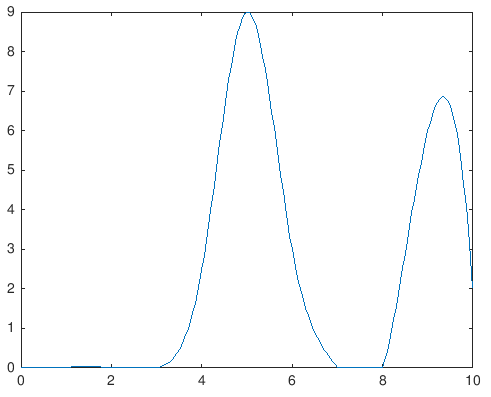
\includegraphics[height=.35\textwidth]{spline_pdf.png}
    \caption{Stetige Wahrscheinlichkeitsverteilung}\label{fig:pdf}
\end{figure}

Die Abbildung \ref{fig:pdf} zeigt beispielhafte eine Dichtefunktion. Für $x=5$ und $x=9$ soll die Wahrscheinlichkeit am größten sein zufällig generiert zu werden. In den Intervallen $[0;2.5]$ und $[6.5,8]$ ist die Dichtefunktion gleich $0$, wodurch Werte innterhalb dieser Intervalle nicht generiert werden können.

Die Dichtefunktion kann nun integriert werden, indem kumulativ der Flächeninhalt für jeden Datenpunkt bestimmt wird. Der Flächeninhalt, der von zwei Punkten eingeschlossen wird, kann nur drei mögliche Formen einnehmen:
\begin{itemize}
    \item Rechtwinkliges Dreieck
    \item Rechteck
    \item Trapez
\end{itemize}
In jedem Fall aber kann der Flächeninhalt mit der Trapezformel näherungsweise berechnet werden. Der Hintegrund ist, dass mithilfe einer Geraden der Breich zwischen den Punkten näherungsweise interpoliert werden kann.\\
Wählt man zwei sukzessive Punkte der stetigen Wahrscheinlichkeitsverteilung $(x_n,y_n)$ und $(x_{n+1},y_{n+1})$, dann ist der Flächeninhalt $A_n$ definiert durch
$$A_n=(x_{n+1}-x_n)*\frac{y_n+y_{n+1}}{2}$$

Wird der Flächheninhalt zwischen allen sukzessiven Punkten berechnet und kumulativ aufaddiert, ist das Ergebnis die Wahrscheinlichkeitsfunktion oder englisch CDF (kumulative distribution function) \cite{denker:2008}. Dies wird in der folgenden Abbildung \ref{fig:cdf} visualisiert.

\begin{figure}[H]
    \centering
    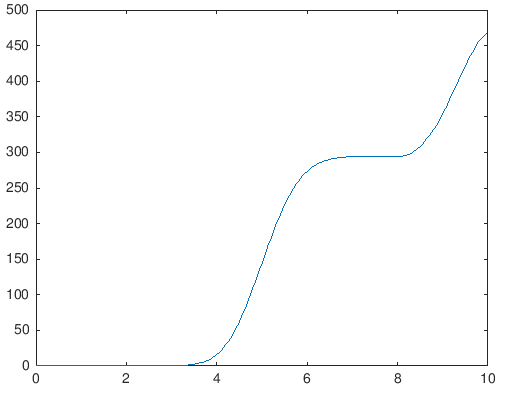
\includegraphics[height=.35\textwidth]{spline_cdf.png}
    \caption{Kumulative Wahrscheinlichkeitsverteilung}\label{fig:cdf}
\end{figure}

Eigentlich gilt für die eingeschlossene Fläche der Dichtefunktion $sum(pdf)=1$. Bei der Modellierung der Wahrscheinlichkeitsverteilung kann nicht gleich garantiert werden, dass die Fläche unter der erstellten Kurve gleich $1$ ist. Dies stellt jedoch kein Problem dar, da die $cdf$ problemlos normiert werden kann, indem jeder y-Wert der berechneten Punkte der $cdf$ durch den gesamten Flächeninhalt der $pdf$ geteilt wird.

\begin{figure}[H]
    \centering
    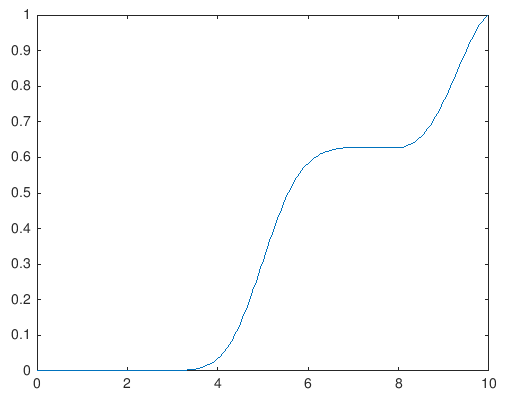
\includegraphics[height=.35\textwidth]{spline_cdf_norm.png}
    \caption{Normierte kumulative Wahrscheinlichkeitsverteilung}\label{fig:cdfnorm}
\end{figure}

Das Ergebnis der Normierung wird in der Abbildung \ref{fig:cdfnorm} gezeigt.
An dieser Stelle wird die Inversionsmethode verwendet, um eine $U(0,1)$-verteilte Zufallsvariable auf eine vorgegebene Wahrscheinlichkeitsfunktion $F$ abzubilden \cite{Inversionsmethode}. Dafür wird ein gleichverteilter Zufallswert auf der vertikalen Achse generiert und der zugehörige Wert auf der Wahrscheinlichkeitsfunktion gesucht. Werte zwischen den Punkten können auch an dieser Stelle linear interpoliert werden. Der erhaltene Zufallswert unterliegt nun der vorgegebenen Wahrscheinlichkeitsverteilung.

\begin{figure}[H]
    \centering
    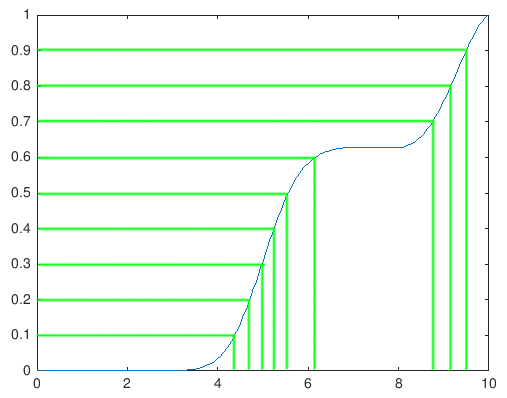
\includegraphics[height=.35\textwidth]{spline_cdf_norm_ex.png}
    \caption{Anwendung der Inversionsmethode}\label{fig:cdfnormex}
\end{figure}

Anschaulich kann die beschriebene Methode in der Abbildung \ref{fig:cdfnormex} betrachtet werden. Durch die grünen Linien wird verdeutlicht, dass ein relativ großer Bereich auf der vetikalen Achse von ca. $0.1$ bis $0.6$ auf einen vergleichsweise kleineren Bereich auf der hoizontalen Achse von ca. $4$ bis $6$ abgebildet wird. Die Autrittswahrscheinlichkeit ist für die Werte $5$ und $9$ am größten.

\subsubsection{Zufallszahlengeneration für stetige Wahrscheinlichkeitsverteilungen}
Die näherungsweise Integration verläuft bei stetigen Wahrscheinlichkeitsverteilung ähnlich. Der Unterschied besteht jedoch darin, dass sukzessive Punkte nicht linear, sondern stufenweise verbunden sind. In diesem Fall kann der Flächeninhalt zwischen sukzessiven Punkten bestimmt werden, indem der Flächeninhalt eines Rechtecks berechnet wird.
Wählt man zwei sukzessive Punkte der diskreten Wahrscheinlichkeitsverteilung $(x_n,y_n)$ und $(x_{n+1},y_{n+1})$, dann ist der Flächeninhalt $A_n$ definiert durch
$$A_n=(x_{n+1}-x_n)*y_n$$

\section{Web Worker}
JavaScript ist im Browser single-threaded. Das bedeutet, dass die Webseite \enquote{einfriert}, wenn eine Berechnung lange benötigt. Es kann also keine Interaktion mit der Seite mehr vorgenommen werden \cite{googledev:webworkers}. Solche Interaktionen sind beispielsweise das Klicken auf Buttons oder das Scrollen der Seite.

Für diese Arbeit muss jedoch eine große Anzahl von Datensätzen generiert werden. Dies soll möglichst schnell geschehen; gleichzeitig soll die Applikation trotzdem bedienbar bleiben und einen Fortschrittsbalken anzeigen.

Um diese Anforderungen umzusetzen, werden sogenannte \textit{Web Worker} verwendet. Web Worker werden in separaten Hintegrundthreads ausgeführt und blockieren dadurch nicht den Hauptthread \cite{mdn:webworkers}. Da JavaScript nicht multithreading-fähig ist, besitzen der Hauptthread und die Web Worker keinen geteilten Adressraum. Es können also keine Objektreferenzen aus dem Hauptthread im Web Worker oder andersherum verwendet werden \cite{mdn:webworkers}.

\subsection{Übertragen von Daten zwischen Workern und Hauptthread}

Die Kommunikation zwischen Hauptthread und Web Workern funktioniert über Nachrichten. Jeder Nachricht können Daten beigefügt werden. Weil keine Referenzen verwendet werden können, werden die Daten kopiert \cite{mdn:webworkers}.

Um komplexe Datentypen zwischen Workern und dem Hauptthread zu übertragen, gibt es mehrere Möglichkeiten:
\begin{itemize}
    \item \textbf{Serialisierung über JSON}: Über die Standardfunktionen \texttt{JSON.stringify()} und \texttt{JSON.parse()} können komplexe Datentypen serialisiert beziehungsweise deserialisiert werden. So kann beispielsweise ein Objekt im Worker serialisiert werden, der entstandene String über \texttt{postMessage()} an den Hauptthread übertragen werden und das Objekt dort deserialisiert werden. Mit dieser Methode können keine zyklischen Objekte (also Objekte, die eine Referenz auf sich selber enthalten) serialisiert werden \cite{mdn:json_stringify}; dies stellt aber im Kontext dieser Arbeit kein Problem dar.
    \item \textbf{Structured Cloning}: Für die Übergabe von Objekten von und zu Workern wurde der Structured Cloning Algorithmus entwickelt. Dieser klont die Objekte und unterstützt dabei auch zyklische Referenzen \cite{mdn:structured_cloning}.
    \item \textbf{Transferables}: Transferable Objects sind Objekte, die zwischen JavaScript-Kon\-texten transferiert werden können. Dabei werden die Objekte nicht kopiert. Stattdessen wird die Referenz auf das Objekt im Ursprungskontext zerstört und im Zielkontext angelegt \cite{googledev:transferables}. Dadurch wird weiterhin eine Threadsicherheit gewährleistet.
\end{itemize}

Auch wenn Transferables in der Theorie die schnellste Art sein sollten, Daten auszutauschen, zeigt sich in der Praxis, dass es stark auf die Art der Daten ankommt, welche Methode die schnellste ist \cite{transferables1, transferables2, transferables3}.

Die generierten Daten werden in der entwickelten Applikation in einem Array von Objekten gespeichert. Jedes Objekt stellt dabei einen einzelnen Datensatz dar, wobei die Schlüssel innerhalb des Objekts die Spaltennamen abbilden.

Arrays sind in JavaScript nicht transferable. Das bedeutet, dass das generierte Array zuerst in einen binären ArrayBuffer überführt werden müsste. Dieser Vorgang macht den Geschwindigkeitsvorteil von Transferables wieder zunichte, so dass entschieden wurde, die generierten Daten letztendlich über den Structured Clone Algorithm zu übertragen.

\subsection{Ablauf der Datengenerierung}

Die Datengenerierung läuft nach folgendem Muster ab:

\begin{enumerate}
    \item Es werden so viele Web Worker gestartet, wie in den Einstellungen festgelegt wurden (standardmäßig 4)
    \item Die Anzahl der zu generierenden Daten wird auf die verschiedenen Worker aufgeteilt. Jeder Worker erhält eine Nachricht mit folgendem Inhalt:
    \begin{itemize}
        \item Modell (Graph), gespeichert von BaklavaJS
        \item Index des ersten zu berechnenden Datensatzes
        \item Index des letzten zu berechnenden Datensatzes
    \end{itemize}
    \item Jeder Worker hat eine eigene Instanz eines BaklavaJS-Editors mit dem Engine-Plugin. Das in der Nachricht enthaltene Modell wird geladen
    \item In einer Schleife werden die Datensätze zwischen Anfangs- und Endindex generiert. Wenn mehr als 10.000 Datensätze generiert werden, werden die Zwischenergebnisse alle 10.000 Datensätze über eine Nachricht an den Hauptthread geschickt. Dadurch wird verhindert, dass der Hauptthread (und damit die gesamte Applikation) einfriert, wenn ein Worker am Ende beispielsweise 500.000 Datensätze an den Hauptthread schickt, welcher die Daten verarbeiten muss.
\end{enumerate}

\section{Dateispeicherung}

Idealerweise sollten die Daten parallel zur Generierung bereits in die Ausgabedatei geschrieben werden. Damit kann die Arbeitsspeicherauslastung gering gehalten werden, was besonders auf Geräten mit kleinem Arbeitsspeicher, wie zum Beispiel günstigen Laptops oder bei Mobilgeräten wichtig ist. Allerdings ist mit JavaScript in Browsern aus Sicherheitsgründen kein direkter Zugriff auf das Dateisystem möglich. Dadurch ist es schwierig, die Datei sequentiell zu schreiben.

Die Bibliothek \textit{StreamSaver.js} versucht, dieses Problem zu lösen \cite{streamsaver}. Dafür benutzt sie einen \textit{Service Worker}. Service Worker haben die Möglichkeit, Webseiten offline verfügbar zu machen, indem sie HTTP-Anfragen abfangen \cite{mdn:serviceworker}. StreamSaver.js nutzt diese Möglichkeit, um einen Download-Stream zu öffnen. Dieser wird vom Browser wie bei einem normalen Dateidownload sequentiell in das Dateisystem geschrieben.

\begin{figure}[H]
    \centering
    \begin{sequencediagram}
        \newthread{mt}{Hauptthread}
        \newinst[1]{sw}{Service Worker}
        \newinst[1]{b}{Browser}

        \begin{call}{mt}{1. Get URL}{sw}{2. URL}\end{call}

        \begin{messcall}{mt}{3. Download URL}{b}
            \begin{call}{b}{4. Fetch URL}{sw}{5. Stream}\end{call}
        \end{messcall}

        \begin{sdblock}{Loop}{}
            \begin{messcall}{mt}{6. Write Data}{sw}
                \begin{messcall}{sw}{
                    \shortstack{7. Write Data \\ to Stream}}{b}\end{messcall}
            \end{messcall}
        \end{sdblock}

        \begin{messcall}{mt}{8. End}{sw}
            \begin{messcall}{sw}{9. Close Stream}{b}\end{messcall}
        \end{messcall}

    \end{sequencediagram}
    \caption{UML-Sequenzdiagramm Download mit StreamSaver.js}
    \label{fig:streamsaverflow}
\end{figure}

\begin{enumerate}
    \item Der Hauptthread initiiert den Vorgang indem er eine Nachricht an den Service Worker schickt
    \item Der Service Worker generiert eine Download-URL und schickt dem Hauptthread eine Nachricht zurück, die die Download-URL und einen speziellen Kommunikationskanal enthält, über den der Hauptthread Daten für diese URL an den Service Worker schicken kann
    \item Der Hauptthread weist den Browser an, einen Download auf die erhaltene URL zu starten
    \item Der Browser schickt eine HTTP-Anfrage an die URL. Der Service Worker erkennt, dass die URL eine von ihm generierte URL ist und fängt die Anfrage ab
    \item Der Service Worker öffnet einen Stream, um dem Browser die Antwort zu schicken
    \item Der Hauptthread schickt über den erhaltenen Kommunikationskanal Daten an den Service Worker
    \item Der Service Worker erhält diese Daten und schreibt sie in den Stream, welcher in Schritt 5 geöffnet wurde
    \item Der Hauptthread beendet die Kommunikation, indem er den speziellen Kommunikationskanal schließt
    \item Der Service Worker erkennt, dass der Kommunikationskanal geschlossen wurde und schließt den Download-Stream. Damit erkennt der Browser, dass der Download abgeschlossen ist und markiert dies entsprechend in der grafischen Benutzeroberfläche des Browsers
\end{enumerate}

Dieser Ansatz hätte es erlaubt, die generierten Daten schon parallel zur Generierung in eine Datei zu schreiben und damit die Arbeitsspeicherauslastung gering zu halten. Leider konnte die Bibliothek in dieser Arbeit nicht zum Laufen gebracht werden; auch eine eigene Umsetzung schlug fehl. Aus diesem Grund werden in der finalen Implementierung dieser Arbeit erst alle Daten in den Arbeitsspeicher geladen und anschließend ein Download auf die Gesamtdatenmenge gestartet. Dies ist mit einfachen JavaScript-Funktionen umsetzbar.